\documentclass{Class/julia}

\usepackage{geometry}
\usepackage{graphicx} % To use \resizebox
\usepackage{array} % For custom column widths
\usepackage{calc} % To use \widthof

\usepackage{siunitx} % Formatting numbers in a table

\usepackage{amsmath}
\usepackage{amsfonts}
\usepackage{subcaption}
\usepackage{threeparttable}
\usepackage{hyperref}
\usepackage{listings}
\usepackage{xcolor}
\usepackage{multirow}
%\usepackage{placeins}
\usepackage{booktabs}
\usepackage{tablefootnote}

\geometry{
    a4paper,
    total={170mm,257mm},
    left=20mm,
    top=20mm,
}

%\author{Julia Maria Wdowinska}
\date{} % Remove date from the title

\begin{document}

\begin{titlepage}
    \centering
    \vfill
    {\scshape\Large University of Milan \par}
    \vspace{0.5cm}
    {\scshape\large Faculty of Political, Economic and Social Sciences \par}
    \vspace{3cm}
    {\huge
    \textbf{A Bayesian Approach to Aggregate Insurance Claim Modeling} \\
    \vspace{0.5cm}
    \large Final Project in the Subject Bayesian Analysis \par}
    \vspace{2cm}
    {\large \textbf{Julia Maria Wdowinska} (43288A) \par}
    {\large \textbf{Edoardo Zanone} (33927A) \par}
    \vspace{0.5cm}
    {\large Data Science for Economics \par}
    {\large II Year \par}
    {\large Master’s Degree \par}
    \vfill
\begin{center}
\begin{figure}[h!]\centering
 
\includegraphics[keepaspectratio=true,scale=0.2]{logo} \\
\end{figure}
\end{center}
\vfill
\begin{center}
{\small{We declare that this material, which we now submit for assessment, is entirely our own work and has not been taken from the work of others, save and to the extent that such work has been cited and acknowledged within the text of our work. We understand that plagiarism, collusion, and copying are grave and serious offences in the university and accept the penalties that would be imposed should I engage in plagiarism, collusion or copying. This assignment, or any part of it, has not been previously submitted by us or any other person for assessment on this or any other course of study.}}
\end{center}
\vfill
    {\large \today \par}
    \vfill
\end{titlepage}

\tableofcontents
%\newpage

\section{Introduction}

\section{Theoretical Considerations}
The goal is to apply Bayesian statistics to our models. The Bayesian approach differs from the classical frequentist one, where, usually, the sample size is large and the parameter \( \theta \) is assumed to be fixed.

In contrast, according to the Bayesian methodology, \( \theta \) is treated as a random variable with prior distribution \( \pi(\theta) \). The information available about the possible values of \( \theta \), prior to observing the data \( \vec y \), is summarized by \( \pi(\theta) \).

Both approaches to statistics have their own strengths and weaknesses, and, in practice, they often complement each other. A common critique of the Bayesian method is the subjectivity involved in choosing a prior distribution. There are various different methods for selecting the right priors. However, as the sample size increases, the influence of the prior diminishes, and the outcomes of the two methods tend to converge. 
Although the classical approach is often computationally easier, it can sometimes produce inconsistent results, especially in the context of hypothesis testing. In contrast, the Bayesian method offers coherent and flexible framework by incorporating prior knowledge and providing full posterior distributions. Even though the choice of the prior may arise potential inconsistencies, Bayesian inference tends to be more advantageous in situations with limited or complex data.
However, in addition to the subjectivity of the priors, Bayesian methods can be computationally intense and complex, moreover, when dealing with complex models or non-conjugate priors. 

Through the use of Bayes' Theorem, the ultimate aim is to find the posterior distribution of our parameter \( \theta \):

\[
\pi(\theta | y) = \frac{f(\vec y | \theta) \pi(\theta)}{\int f(\vec y | \theta) \pi(\theta) \, d\theta},
\]
where \(f(\vec y|\vec \theta)\) is the likelihood function. Given that the denominator is constant with respect to \(\theta\) it is possible to simplify the expression to :
\[
\pi(\theta|\vec y) \propto \pi(\theta)f(\vec y | \theta).
\]

Usually, to simplify computations, it is common to use conjugate distributions. A family \( \mathcal{F} \) is said to be conjugate to the likelihood if, for every prior that belongs to \( \mathcal{F} \), the posterior distribution of \( \theta \) also belongs to the same family.

When the posterior distributions are analytically intractable, the use of \textit{Markov Chain Monte Carlo} (MCMC) methods becomes essential. The main goal of MCMC is to draw samples from a probability distribution from which direct sampling is difficult.

Among the different algorithms available for implementing MCMC, two are considered here: the \textit{Gibbs sampler} and the \textit{Metropolis-Hastings algorithm}.

The first algorithm mentioned aims to find the full conditional posterior distributions starting from the joint or marginal posterior distributions. It is particularly efficient when these conditional distributions have a closed form. Hence, conjugate priors are often preferred. The algorithm proceeds through a clear and structured series of steps:

\begin{itemize}
  \item Fix the initial value of the parameter \( \vec\theta^{(0)} = (\theta^{(0)}_1,\ldots,\theta^{(0)}_p) \) and initialize the iteration counter as \( m = 1 \);
  \item Obtain \( \theta^{(0)} \) such that \( \pi(\theta^{(m)}1|\theta^{(m-1)}_2,\ldots,\theta^{(m-1)}_p, \vec y) \propto f(\vec y|\vec\theta^{(m-1)})\pi(\vec\theta^{(m-1)} \), now draw \(\theta^{(m)}_2 \) from the full conditional posterior distribution \( \pi(\theta^{(m)}_2|\theta^{(m)}_1, \theta^{(m-1)}_3\ldots,\theta^{(m-1)}_p, \vec y) \), and so on until \(\pi(\theta^{(m)}_p|\theta^{(m)}_1,\ldots,\theta^{(m)}{p-1}, \vec y)\);
  \item Increment the counter from \( m \) to \( m + 1 \) and return to the first step.
\end{itemize}

The Metropolis-Hastings algorithm, on the other hand, is used when the full conditional posterior distribution is not in closed form. Suppose a realization from the full conditional distribution is desired: a proposal distribution with density \( q(\theta^* | \theta) \) is used to generate candidate values \( \theta^* \) from the current state \( \theta \). This algorithm also follows a clear and structured procedure:

\begin{itemize}
  \item Initialize the chain \( \theta_0 \) and the iteration counter;
  \item Generate a candidate value \( \theta^* \) from a proposal distribution \( q(\theta^* | \theta) \);
  \item Evaluate the acceptance probability \( p(\theta^, \theta^{(j-1)}) \) of the proposed draw \( p(\theta^,\theta^{(j-1)})=min(1,\frac{\pi(\theta^|\vec y)}{\pi(\theta^{(j-1)}|\vec y)}\frac{q(\theta^{(j-1)}|\theta^)}{p(\theta^*|\theta^{(j-1)})}\);
  \item Draw a uniform value \( U \sim U(0,1) \), set \( \theta^{(j)} = \theta^* \) if \( U < p(\theta^*, \theta^{(j-1)}) \), otherwise set \( \theta^{(j)} = \theta^{(j-1)} \);
  \item Update the iteration counter and return to the first step.
\end{itemize}

After running the chain, the successive samples are likely to be correlated. Therefore, to obtain a random sample, a thinning process is applied, which consists of keeping one iteration and discarding the following \( m \).

Finally, the chains must run long enough to reach equilibrium, a phase known as \textit{burn-in}.

There are several methods to determine whether a chain is converging adequately. 
Two general approaches exist: one involves running a single chain for a larger number of iterations, while the other involves running multiple chains for a shorter period of time.
Various diagnostics to check if the chain actually reached convergence have been developed, including visual inspection, the Gelman-Rubin test and the Geweke diagnostic.

Visually inspection consist in assessing how well the chain mixes or moves through the parameter space. If the chain moves slowly then the convergence will also be slow. It's important to inspect all the model parameters, since some may converge while others do not. The traceplot, which shows sampled parameter values over iterations, helps detect poor mixing. Thanks to this visualization it is possible to see if a chain get stuck in a certain area of the parameter space, which is the result of a bad mixing.  Another useful tool is the running mean plot, which plots the cumulative average of the samples across iterations and helps evaluate stability over time. 

Looking at the autocorrelation function (A.C.F) can help assessing the convergence. It represents the correlation among the draws of the Markov Chain. High autocorrelation implies strong dependence and slow mixing. In such cases, thinning can help reducing the correlation.

The Gelman-Rublin Test, which works with multiple chains, follows predetermined steps:
\begin{itemize}
    \item Run the m different chains of length 2N, where N is equal to the number of iterations of the MCMC algorithm.
    \item Discard the number of the burn-in iterations (the first N draws?) 
    \item Compute the within-chain variance and the between-chain variance, which are, respectively, \(W=\frac{1}{m}\sum^m_{j=1}(s^2_j)\) and \(B=\frac{N}{m-1}\sum^m_{j=1}(\overline{\theta_j}-\overline{\overline{\theta}})^2\), where \(s^2_j=\frac{1}{N-1}\sum^N_{i=1}(\theta_{ij}-\overline{\theta_j})^2, \overline{\theta_j}=\frac{1}{N}\sum^N_{i=1}(\theta_{ij}\)) and \(\overline{\overline{\theta}}=\frac{1}{N}\sum^m_{j=1}\overline{\theta_j}\)
    \item Compute the estimated variance of the parameter as the weighted average between the sum of between-variance anche within-variance \(\hat{var}(\theta)=(1-\frac{1}{N})W+\frac{1}{N}B\)
    \item Calculate the Potential Scale Reduction factor \(\hat{R}=\sqrt{\frac{\hat{var}(\theta)}{W}}\).
\end{itemize}
When \(\hat{R}\) is larger than 1.2 it is better to run the chain for a larger number of iterations in order to improve the convergence of the algorithm. 

Differently from the Gelman-Rubin, the Geweke Diagnostic test works with a single chain. It takes two non-overlapping parts of the chain of each parameter. The two parts, by default, are the first 0.1 and the last 0.5 of the Markov chain. The Geweke test compares the means of both parts, using a difference of means test to see if the two part of the chain care from the same distributions. The test statistic is a \(N(0,1)\). If the absolute value of the statistic is less than 1.96 then there is no problem with the chain convergence.

\section{Replication of Dudley 2006}

The first objective of this project was to replicate the analysis conducted by \textit{dudley2006bayesian}. The dataset used comprises insurance claim amounts exceeding 1.5 million over a period of five years from an automobile insurance portfolio. The data, originally presented in Rytgaard (1990), is shown in Table 1.

\begin{table}[!ht]
\centering
\footnotesize
\setlength{\tabcolsep}{5pt}
\caption{Insurance Claim Amounts Exceeding 1.5 Million (Data from Rytgaard, 1990)}
\label{tab:1}
\begin{threeparttable}
\begin{tabular}{
>{\raggedright\arraybackslash}p{\widthof{Year}}
*{5}{S[table-format=2.3]}
}
\hline
\textbf{Year} & \multicolumn{5}{c}{\textbf{Claim Amounts (in millions)}} \\ \hline
1 & 2.495 & 2.120 & 2.095 & 1.700 & 1.650 \\
2 & 1.985 & 1.810 & 1.625 & \textendash & \textendash \\
3 & 3.215 & 2.105 & 1.765 & 1.715 & \textendash \\
4 & \textendash & \textendash & \textendash & \textendash & \textendash \\
5 & 19.180 & 1.915 & 1.790 & 1.755 & \textendash \\ \hline
\end{tabular}
\begin{tablenotes}
\footnotesize
\item The threshold of 1.5 million corresponds to the retention level of an excess-of-loss insurance policy\tablefootnote{To manage risk exposure, insurers frequently employ reinsurance strategies, which help reduce their financial liability on large claims. Under such arrangements, if a claim amount \( y \) exceeds a predetermined threshold \( d \) (the retention), the insurer is responsible only for paying up to \( d \), while any excess \( y - d \) is covered by the reinsurer.}.
\end{tablenotes}
\end{threeparttable}
\end{table}

To model this dataset within a Bayesian framework, assumptions about the distributions of both the number of claims in year \( t \) (\( N_t \)) and the amount of the \( i \)-th claim in year \( t \) (\( Y_{i,t} \)) were necessary. Claims were assumed to occur randomly and independently at a constant rate over time, so \( N_t \) was modeled using a Poisson distribution. A Pareto distribution was chosen for \( Y_{i,t} \), as a heavy-tailed loss distribution was needed to account for the fact that individual claim amounts are positive and may include large outliers. That is,
\begin{align*}
N_t &\sim \text{Poisson}(\theta), \quad 0 < \theta < \infty, \\
Y_{i,t} &\sim \text{Pareto}(\alpha, \beta), \quad \alpha > 0, \quad 0 < \beta < y.
\end{align*}

\noindent The \text{Pareto}\((\alpha, \beta)\) distribution with support \( [\beta, \infty) \) was particularly suitable in this context, as we were modeling claim amounts exceeding a certain threshold.

In addition, the following assumptions were made:

\begin{itemize}
\item \( N_t \) are independently and identically distributed (i.i.d.) across \( t \),
\item \( Y_{i,t} \) are i.i.d.\ across both \( i \) and \( t \),
\item \( N_t \) and \( Y_{i,t} \) are independent for all \( i \) and \( t \).
\end{itemize}

\noindent Under these assumptions, the aggregate claim amount in year \( t \), denoted by
\[
S_t = Y_{1,t} + Y_{2,t} + \cdots + Y_{N_t,t},
\]
follows a compound Poisson distribution, since it represents the sum of independent Pareto-distributed random variables. [This is wrong?]

Next, prior distributions for the parameters \( \alpha \), \( \beta \), and \( \theta \) were specified. Due to limited prior knowledge about their true values—beyond the assumption that they are strictly positive—vague Gamma priors were chosen:
\[
\alpha \sim \text{Gamma}(1, 0.0001), \quad \beta \sim \text{Gamma}(1, 0.0001), \quad \theta \sim \text{Gamma}(1, 0.0001),
\]
with the constraint \( 0 < \beta < \min\{y_{i,t}\} \) to ensure validity of the Pareto distribution. Each of these Gamma priors has a variance of \(10^8\), implying minimal prior influence so that most of the information about the parameters is derived from the dataset. Additionally, the Gamma distribution is conjugate to both the Poisson and Pareto likelihoods, facilitating analytical tractability in Bayesian inference.

Finally, the posterior distributions were derived. First, the joint posterior distribution of \( (\alpha, \beta) \) was obtained via Bayes' theorem\footnote{Here, assuming that \( \alpha \) and \( \beta \) are independent, the joint prior \( \pi(\alpha, \beta) \) was computed as \( \pi(\alpha) \cdot \pi(\beta) \).}:
\begin{align*}
\pi(\alpha, \beta \mid \mathbf{y}) &\propto \pi(\alpha) \cdot \pi(\beta) \cdot f(\mathbf{y} \mid \alpha, \beta) \\
&\propto 0.0001 \cdot \exp(-0.0001 \alpha) \cdot 0.0001 \cdot \exp(-0.0001 \beta) \cdot \prod_{i=1}^{n} \frac{\alpha \beta^\alpha}{y_i^{\alpha+1}} \\
&\propto \exp(-0.0001 \alpha) \cdot \exp(-0.0001 \beta) \cdot \alpha^n \cdot \beta^{n \alpha} \left( \prod_{i=1}^{n} y_i \right)^{-(\alpha + 1)} \\
&\propto \alpha^n \cdot \exp(-0.0001 \alpha) \cdot \left( \prod_{i=1}^{n} y_i \right)^{-\alpha} \cdot \beta^{n \alpha} \cdot \exp(-0.0001 \beta) \\
&\propto \alpha^n \cdot \exp\left( - \left( 0.0001 + \sum_{i=1}^{n} \ln(y_i) \right) \alpha \right) \cdot \beta^{n \alpha} \cdot \exp(-0.0001 \beta)
\end{align*}

\noindent As a result, the full conditional posterior distributions of \( \alpha \) and \( \beta \) were as follows:
\begin{align*}
\pi(\alpha \mid \beta, \mathbf{y}) &\propto \alpha^n \cdot \exp\left( - \left( 0.0001 - n \ln(\beta) + \sum_{i=1}^{n} \ln(y_i) \right) \alpha \right) \\
\pi(\beta \mid \alpha, \mathbf{y}) &\propto \beta^{n \alpha} \cdot \exp(-0.0001 \beta)
\end{align*}

\noindent which implied that:
\begin{align*}
\alpha \mid \beta, \mathbf{y} &\sim \text{Gamma}\left(n+1, \sum_{i=1}^{n} \ln(y_i) - n \ln(\beta) + 0.0001\right), \\
\beta \mid \alpha, \mathbf{y} &\sim \text{Gamma}(n \alpha + 1, 0.0001)
\end{align*}

Similarly, the posterior distribution of \( \theta \) was obtained via Bayes' theorem:
\begin{align*}
\pi(\theta \mid \mathbf{n}) &\propto \pi(\theta) \cdot f(\mathbf{n} \mid \theta) \\
&\propto \exp(-0.0001 \theta) \cdot \prod_{t=1}^{T} \left( \theta^{n_t} \cdot \exp(-\theta) \right) \\
&\propto \exp(-0.0001 \theta) \cdot \theta^{\sum_{t=1}^{T} n_t} \cdot \exp(-5 \theta) \\
&\propto \exp(-5.0001 \theta) \cdot \theta^{\sum_{t=1}^{T} n_t}
\end{align*}

\noindent which implied that:
\[
\theta \mid \mathbf{n} \sim \text{Gamma}\left( \sum_{t=1}^{T} n_t + 1, 5.0001 \right)
\]

Since all three posterior distributions were standard distributions, the Gibbs sampling method was employed to draw realizations from them. This was implemented using the \texttt{JAGS} program, which was called from within~\texttt{R}. Three Markov chains were run in parallel. The initial values of \( \alpha \), \( \beta \), and \( \theta \) were chosen to be well-dispersed~and are presented in Table~\ref{tab:2}.

\begin{table}[!ht]
\centering
\footnotesize
\setlength{\tabcolsep}{5pt}
\caption{Initial Parameter Values}
\label{tab:2}
\begin{tabular}{
>{\raggedright\arraybackslash}p{\widthof{Chain}}
*{3}{S[scientific-notation=true, table-format=1.5e1]}
}
\hline
\textbf{Chain} & \( \alpha \) & \( \beta \) & \( \theta \) \\ \hline
1 & 1e-5 & 1e-5 & 1e-5 \\
2 & 1e5 & 1 & 1e5 \\
3 & 3.076 & 1.625 & 3.200 \\ \hline
\end{tabular}
\end{table}

The burn-in period was set to 20,000 iterations. The statistics computed over the results of the subsequent 30,000 iterations are presented in Table~\ref{tab:3}. A comparison with the statistics reported by Dudley shows a close match, indicating that the model was properly specified and the Gibbs sampler was executed correctly.

\begin{table}[!ht]
\centering
\footnotesize
\setlength{\tabcolsep}{5pt}
\caption{Posterior Statistics}
\label{tab:3}
\begin{threeparttable}
\begin{tabular}{
>{\raggedright\arraybackslash}p{\widthof{\( E[Y] \)}}
*{2}{S[table-format=1.3]}
>{\raggedright\arraybackslash}p{\widthof{\textbf{95\% Bayesian Credible Interval}}}
}
\hline
 & \textbf{Mean} & \textbf{Standard Deviation} & \textbf{95\% Bayesian Credible Interval} \\ \hline
\( \alpha \) & 3.079 & 0.763 & (1.771, 4.741) \\
\( \beta \) & 1.592 & 0.035 & (1.498, 1.624) \\
\( \theta \) & 3.396 & 0.821 & (1.982, 5.192) \\
\( E[Y] \) & 2.499 & 0.621 & (2.024, 3.621) \\ \hline
\end{tabular}
\begin{tablenotes}
\footnotesize
\item Note:\ \( E[Y] \) was calculated for each simulated set of parameters \( \alpha \) and \( \beta \), and from these values, the mean, standard deviation, and 95\% Bayesian credible interval were subsequently computed.
\end{tablenotes}
\end{threeparttable}
\end{table}

In addition, density plots were generated for each of the parameters and for \( E[Y] \), as presented in Figure~\ref{fig:1}. The resulting densities for the parameters resemble Gamma distributions, with the density of \( \beta \) appropriately truncated at \( \min\{y_{i,t}\} = 1.625 \). The density plot for \( E[Y] \) displays a right-skewed distribution that permits very large values, albeit with very low probability---consistent with expectations.

\begin{figure}[!ht]
    \centering
    \begin{minipage}{0.45\textwidth}
        \centering
        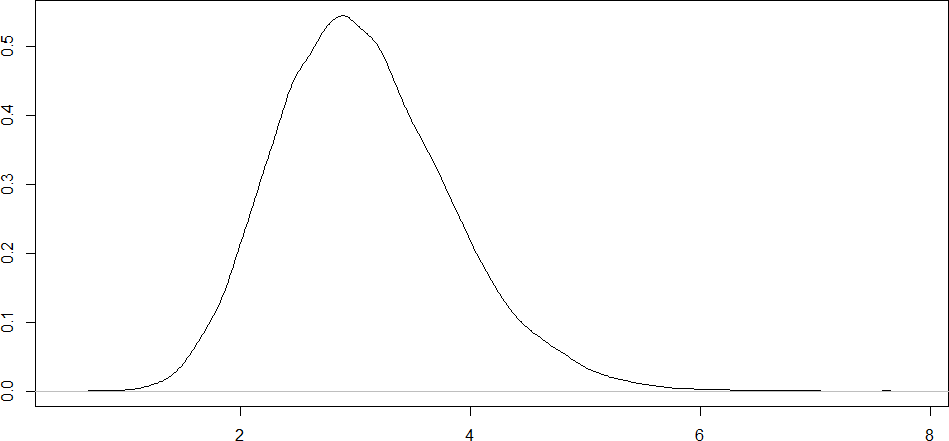
\includegraphics[width=\linewidth]{rytgaard1990/density_alpha.png}
        \subcaption{\( \alpha \)}
    \end{minipage}%
    \hfill
    \begin{minipage}{0.45\textwidth}
        \centering
        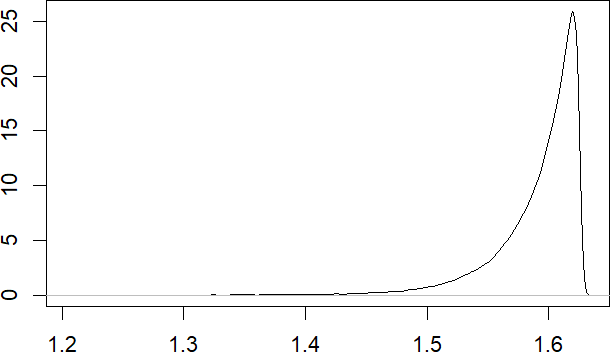
\includegraphics[width=\linewidth]{rytgaard1990/density_beta.png}
        \subcaption{\( \beta \)}
    \end{minipage} \\
    
%    \vspace{0.5cm}
    
    \begin{minipage}{0.45\textwidth}
        \centering
        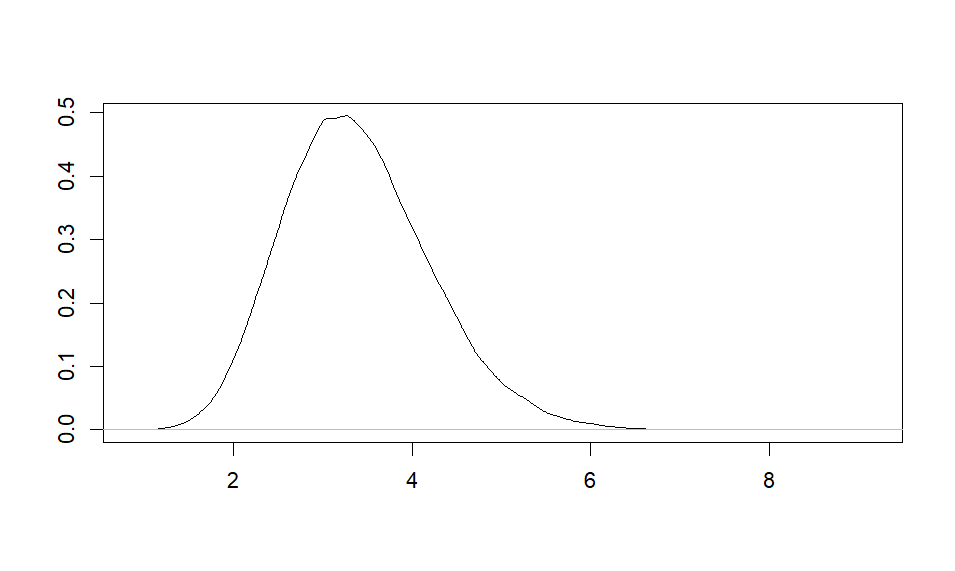
\includegraphics[width=\linewidth]{rytgaard1990/density_theta.png}
        \subcaption{\( \theta \)}
    \end{minipage}%
    \hfill
    \begin{minipage}{0.45\textwidth}
        \centering
        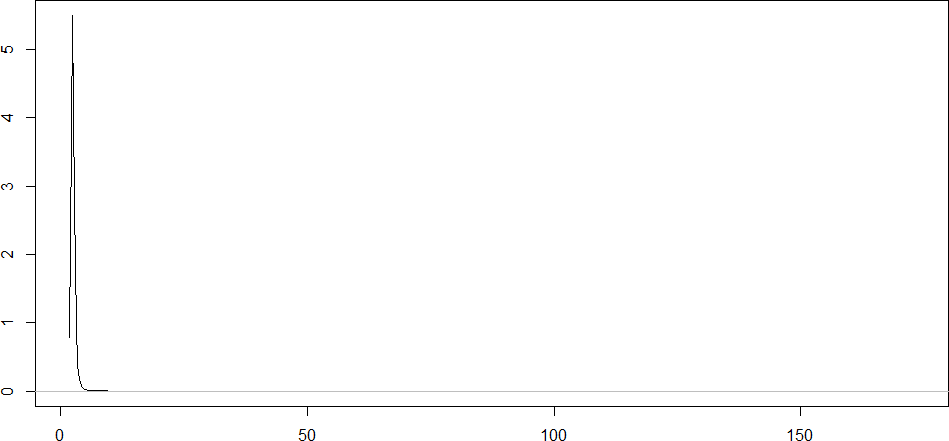
\includegraphics[width=\linewidth]{rytgaard1990/density_E_y.png}
        \subcaption{\( E[y] \)}
    \end{minipage}
    
    \caption{Posterior Densities}
    \label{fig:1}
\end{figure}

The posterior means of \( \alpha \) and \( \beta \) were used as parameters of the Pareto distribution, and the corresponding cumulative distribution function (CDF) was plotted against the empirical cumulative data (\( y_{i,t} \)). Similarly, the posterior mean of \( \theta \) was used as the parameter of the Poisson distribution, and its CDF was plotted against the empirical cumulative data (\( n_t \)).

\begin{figure}[!ht]
    \centering
    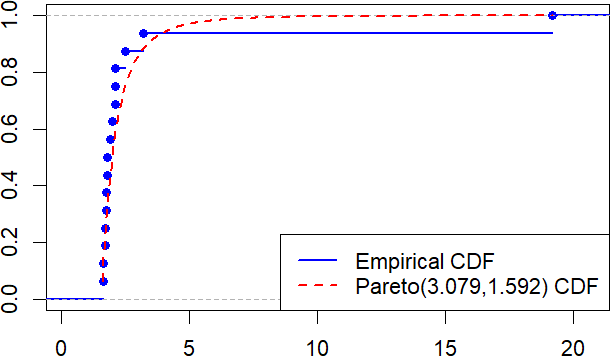
\includegraphics[width=0.8\textwidth]{rytgaard1990/empirical_vs_pareto.png}
    \caption{Empirical vs.\ Fitted Pareto CDF}
    \label{fig:2}
\end{figure}

\begin{figure}[!ht]
    \centering
    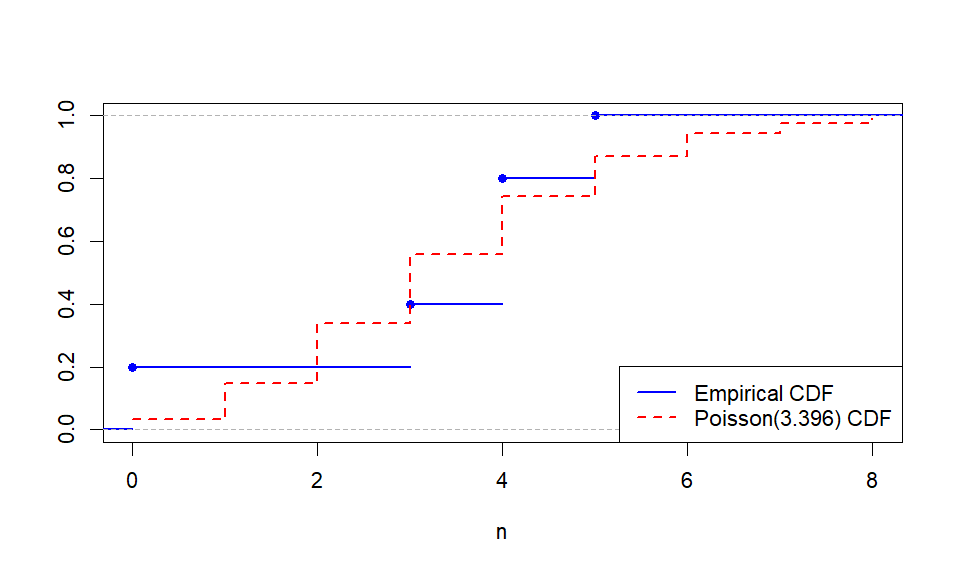
\includegraphics[width=0.8\textwidth]{rytgaard1990/empirical_vs_poisson.png}
    \caption{Empirical vs.\ Fitted Poisson CDF}
    \label{fig:3}
\end{figure}

The Pareto\((3.079,\,1.592)\) distribution provides a close fit to the empirical data. The Poisson\((3.396)\) distribution also fits the observed frequencies quite well.

Throughout all computations, a burn-in period of 20{,}000 iterations was applied, with only samples from iterations 20{,}001 to 50{,}000 retained for analysis. This approach followed the assumptions made by Dudley. However, it is essential to verify that the chains have indeed converged to a stationary distribution after discarding the initial samples. The first method of assessment involves visual inspection. Figure~\ref{fig:4} presents trace plots for all three parameters, showing the sampled values across iterations. These plots indicate good mixing, suggesting that the chains have converged.

\begin{figure}[!ht]
    \centering
    \begin{subfigure}{0.45\textwidth}
        \centering
        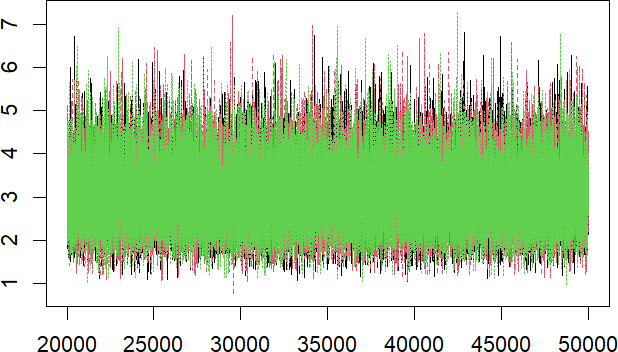
\includegraphics[width=\textwidth]{rytgaard1990/trace_alpha.png}
        \caption{\( \alpha \)}
    \end{subfigure}
    \hfill
    \begin{subfigure}{0.45\textwidth}
        \centering
        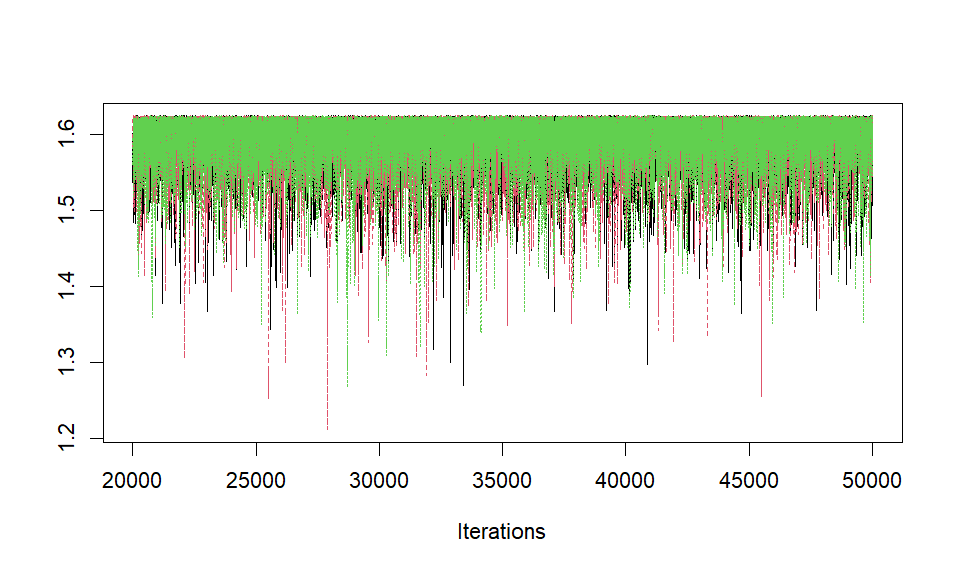
\includegraphics[width=\textwidth]{rytgaard1990/trace_beta.png}
        \caption{\( \beta \)}
    \end{subfigure}

    \vspace{1em}

    \begin{subfigure}{0.45\textwidth}
        \centering
        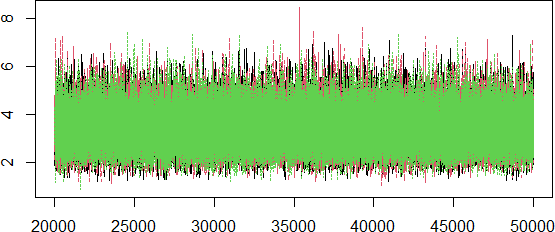
\includegraphics[width=\textwidth]{rytgaard1990/trace_theta.png}
        \caption{\( \theta \)}
    \end{subfigure}

    \caption{Trace Plots}
    \label{fig:4}
\end{figure}

The convergence of the chains was also assessed using the Gelman--Rubin diagnostic. The diagnostic was applied to the post-burn-in iterations (20,001–50,000), and the results are summarized in Table~\ref{tab:4}.

\begin{table}[!ht]
\centering
\footnotesize
\caption{Potential Scale Reduction Factors (Gelman--Rubin Diagnostic)}
\label{tab:4}
\begin{tabular}{
  >{\raggedright\arraybackslash}p{\widthof{\textbf{Multivariate PSRF}}}
  *{2}{S[table-format=1.2]}
}
\hline
\textbf{Parameter} & \textbf{Point Estimate} & \textbf{Upper C.I.} \\
\hline
\( \alpha \) & 1.00 & 1.00 \\
\( \beta \)  & 1.00 & 1.00 \\
\( \theta \) & 1.00 & 1.00 \\
\hline
\textbf{Multivariate PSRF} & \multicolumn{2}{c}{1.00} \\
\hline
\end{tabular}
\end{table}

\noindent All univariate potential scale reduction factors (PSRFs) have point estimates and upper confidence bounds at 1.00. The multivariate PSRF is also equal to 1.00. These values suggest that the Markov chains have likely converged, both for individual parameters and jointly.

Figure~\ref{fig:5} shows how the univariate PSRF point estimates evolve with increasing iterations. Throughout all iterations, all estimates remain below 1.1, which is commonly considered an acceptable threshold for convergence. This further confirms that the chains have likely reached a stable distribution.

\begin{figure}[!ht]
    \centering
    \begin{subfigure}{0.45\textwidth}
        \centering
        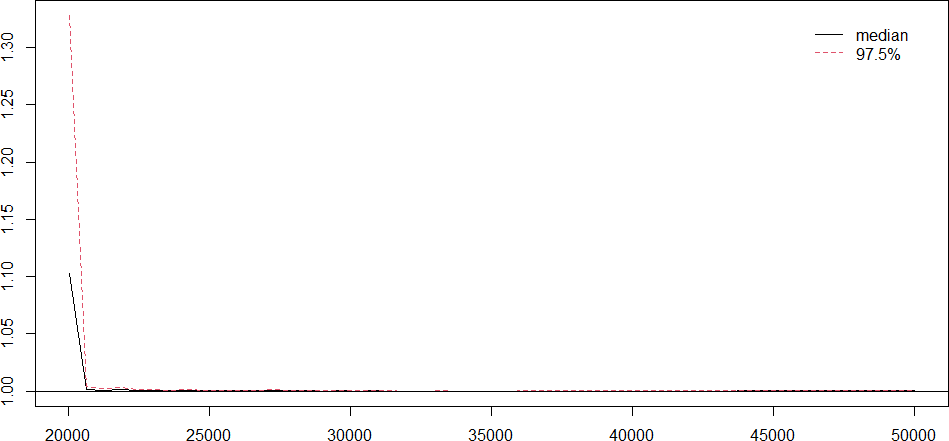
\includegraphics[width=\textwidth]{rytgaard1990/gelman_alpha.png}
        \caption{\( \alpha \)}
    \end{subfigure}
    \hfill
    \begin{subfigure}{0.45\textwidth}
        \centering
        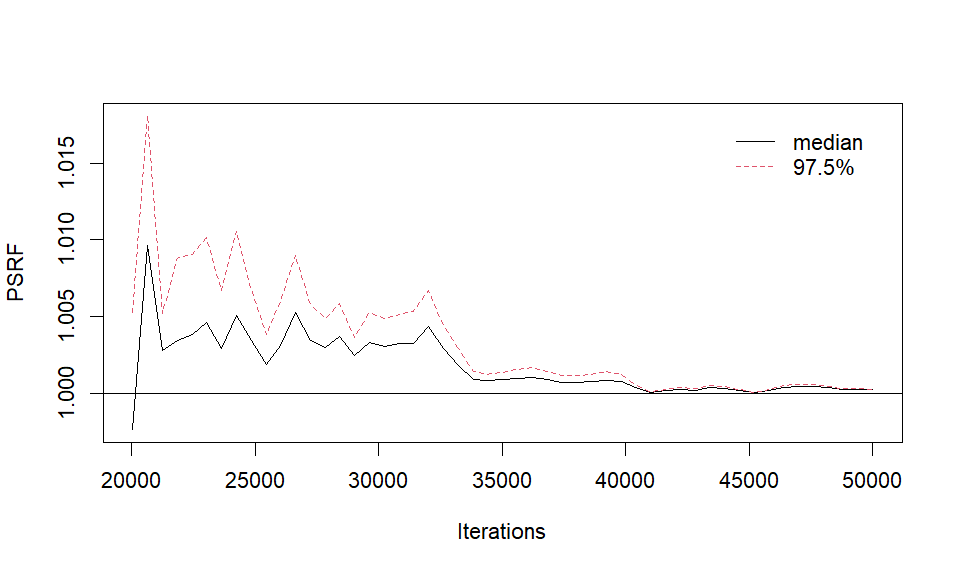
\includegraphics[width=\textwidth]{rytgaard1990/gelman_beta.png}
        \caption{\( \beta \)}
    \end{subfigure}

    \vspace{1em}

    \begin{subfigure}{0.45\textwidth}
        \centering
        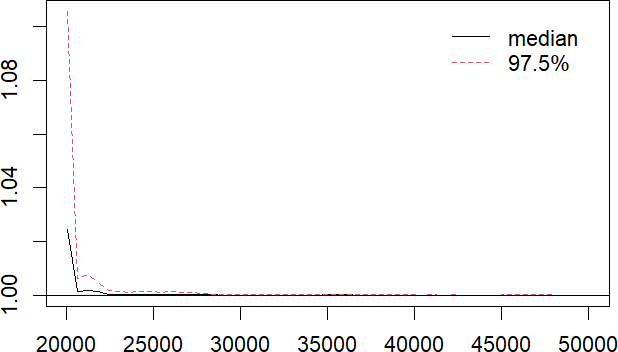
\includegraphics[width=\textwidth]{rytgaard1990/gelman_theta.png}
        \caption{\( \theta \)}
    \end{subfigure}

    \caption{PSRF Values (Gelman--Rubin Diagnostic)}
    \label{fig:5}
\end{figure}

In addition, autocorrelation plots were generated for all three parameters (see Figure~\ref{fig:6}), and values at lags 1 through 10 are reported in Table~\ref{tab:5}. Several high autocorrelations were observed, particularly for \( \beta \), which motivated the use of a thinning interval of 10 iterations, as suggested by Dudley.

\begin{figure}[!ht]
    \centering
    \begin{subfigure}{0.45\textwidth}
        \centering
        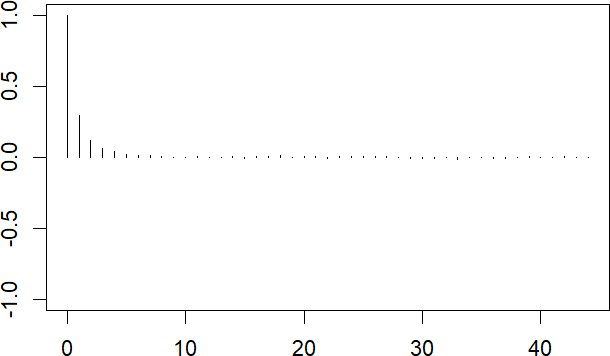
\includegraphics[width=\textwidth]{rytgaard1990/acf_alpha.png}
        \caption{\( \alpha \)}
    \end{subfigure}
    \hfill
    \begin{subfigure}{0.45\textwidth}
        \centering
        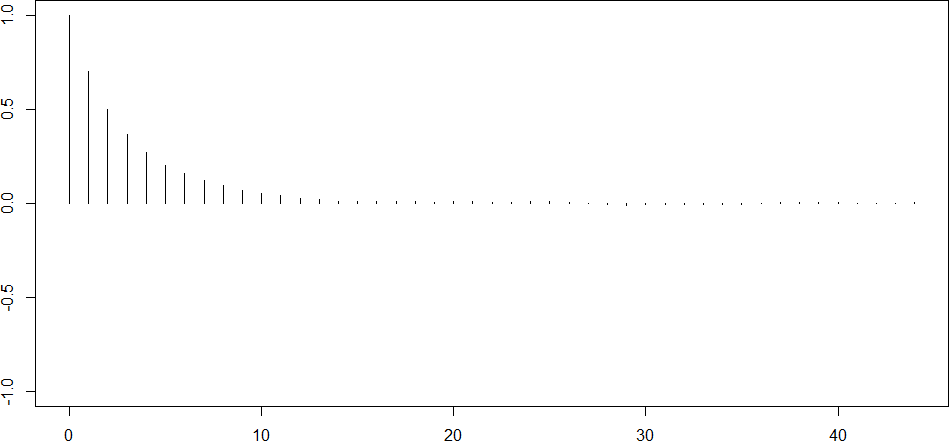
\includegraphics[width=\textwidth]{rytgaard1990/acf_beta.png}
        \caption{\( \beta \)}
    \end{subfigure}

    \vspace{1em}

    \begin{subfigure}{0.45\textwidth}
        \centering
        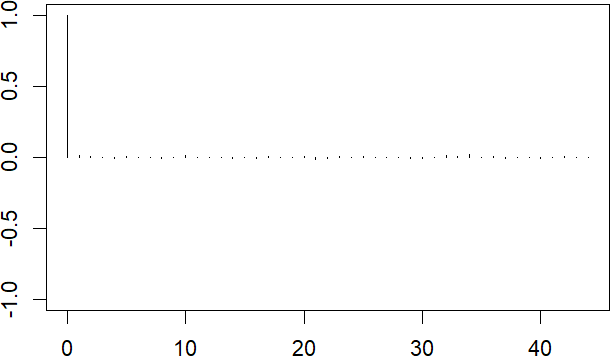
\includegraphics[width=\textwidth]{rytgaard1990/acf_theta.png}
        \caption{\( \theta \)}
    \end{subfigure}

    \caption{Autocorrelation Plots}
    \label{fig:6}
\end{figure}

\begin{table}[!ht]
\centering
\footnotesize
\setlength{\tabcolsep}{5pt}
\caption{Autocorrelations at Lags 1--10}
\label{tab:5}
\begin{tabular}{
>{\raggedright\arraybackslash}p{\widthof{\textbf{Lag}}}
*{3}{S[table-format=-1.3]}
}
\hline
\textbf{Lag} & \( \alpha \) & \( \beta \) & \( \theta \) \\
\hline
1  & 0.297 & 0.705 & 0.003 \\
2  & 0.119 & 0.509 & 0.005 \\
3  & 0.061 & 0.373 & -0.005 \\
4  & 0.036 & 0.278 & -0.004 \\
5  & 0.023 & 0.210 & 0.001 \\
6  & 0.016 & 0.161 & -0.002 \\
7  & 0.010 & 0.126 & -0.004 \\
8  & 0.009 & 0.102 & -0.004 \\
9  & 0.002 & 0.081 & -0.001 \\
10 & 0.007 & 0.065 & 0.004 \\
\hline
\end{tabular}
\end{table}

Consequently, the chains were rerun with this thinning. Figure~\ref{fig:7} presents the corresponding trace plots, and Figure~\ref{fig:8} shows the updated autocorrelation plots. The trace plots indicate that the chains have mixed well, and all autocorrelation values at lags 2, 3, and beyond have become negligible.

\begin{figure}[!ht]
    \centering
    \begin{subfigure}{0.45\textwidth}
        \centering
        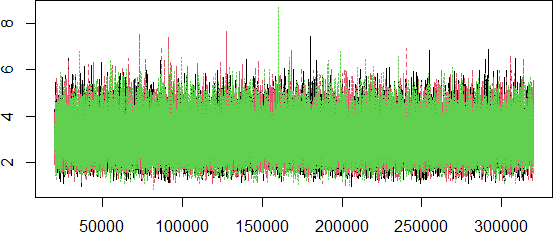
\includegraphics[width=\textwidth]{rytgaard1990/trace_after_thinning_alpha.png}
        \caption{\( \alpha \)}
    \end{subfigure}
    \hfill
    \begin{subfigure}{0.45\textwidth}
        \centering
        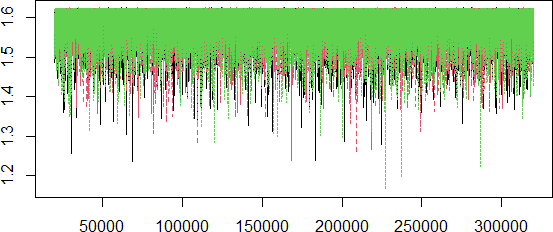
\includegraphics[width=\textwidth]{rytgaard1990/trace_after_thinning_beta.png}
        \caption{\( \beta \)}
    \end{subfigure}

    \vspace{1em}

    \begin{subfigure}{0.45\textwidth}
        \centering
        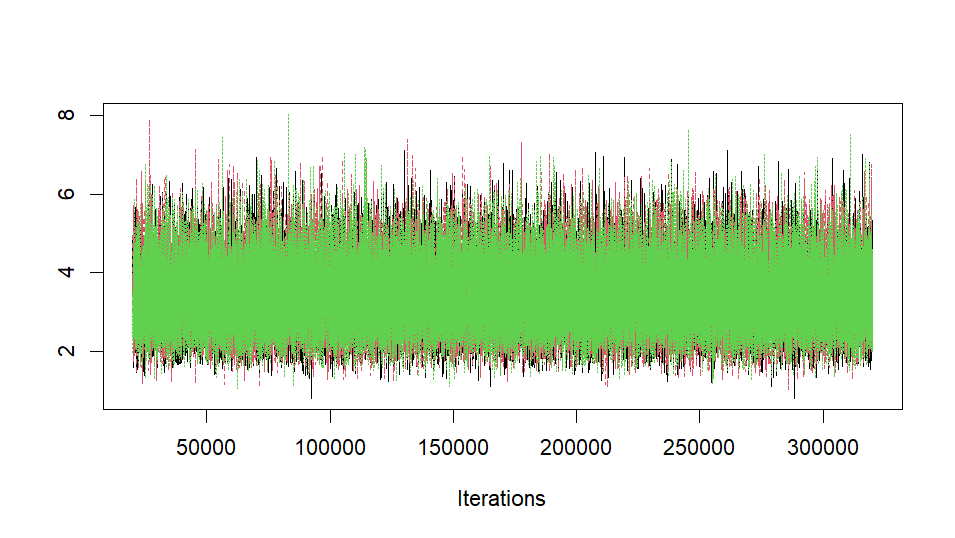
\includegraphics[width=\textwidth]{rytgaard1990/trace_after_thinning_theta.png}
        \caption{\( \theta \)}
    \end{subfigure}

    \caption{Trace Plots After Thinning}
    \label{fig:7}
\end{figure}

\begin{figure}[!ht]
    \centering
    \begin{subfigure}{0.45\textwidth}
        \centering
        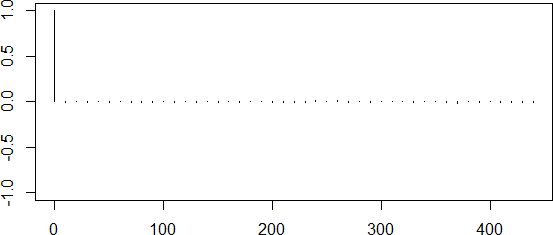
\includegraphics[width=\textwidth]{rytgaard1990/acf_after_thinning_alpha.png}
        \caption{\( \alpha \)}
    \end{subfigure}
    \hfill
    \begin{subfigure}{0.45\textwidth}
        \centering
        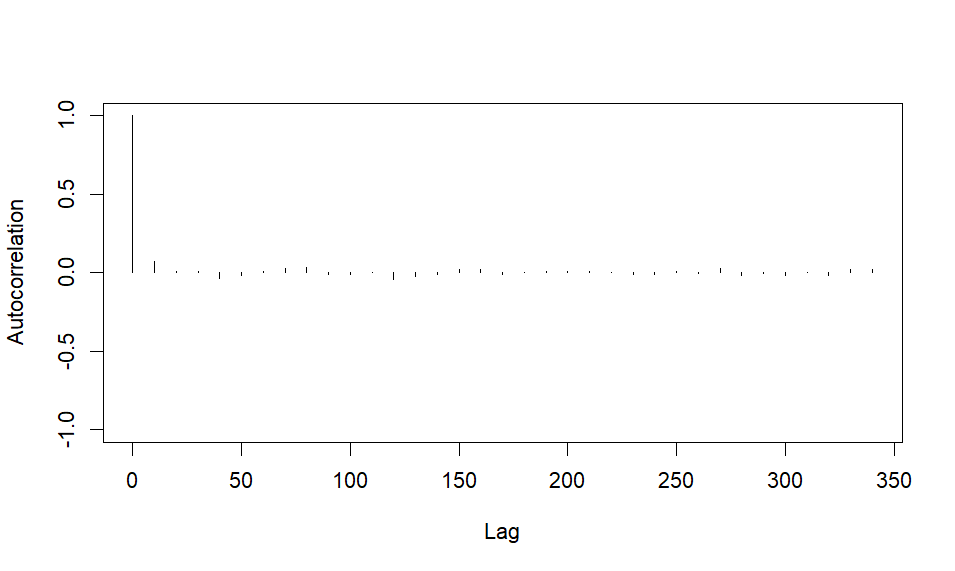
\includegraphics[width=\textwidth]{rytgaard1990/acf_after_thinning_beta.png}
        \caption{\( \beta \)}
    \end{subfigure}

    \vspace{1em}

    \begin{subfigure}{0.45\textwidth}
        \centering
        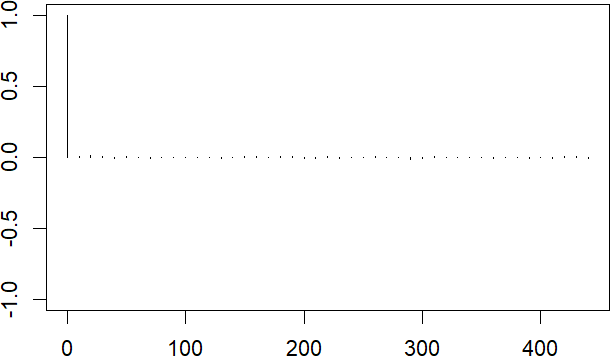
\includegraphics[width=\textwidth]{rytgaard1990/acf_after_thinning_theta.png}
        \caption{\( \theta \)}
    \end{subfigure}

    \caption{Autocorrelation Plots After Thinning}
    \label{fig:8}
\end{figure}

Since the ultimate goal of the analysis was to predict the values of \( S_t \), the posterior predictive distribution was employed. For a variable \( z \), this distribution is defined as:

\[
\pi(z \mid \mathbf{y}) = \int_{\Theta} f(z \mid \mathbf{\phi}) \, \pi(\mathbf{\phi} \mid \mathbf{y}) \, d\mathbf{\phi}
\]

\noindent where \( \mathbf{\phi} = (\alpha, \beta, \theta) \), \( \pi(\mathbf{\phi} \mid \mathbf{y}) \) is the posterior distribution of \( \mathbf{\phi} \), and \( f(z \mid \mathbf{\phi}) \) is the likelihood of \( z \) given \( \mathbf{\phi} \). This approach accounts for the uncertainty in \( \mathbf{\phi} \) by integrating over its possible values, weighted by their posterior probabilities.

Let \( \mathbf{n} \) denote the observed data and \( N_f \) represent a future observation. Then the posterior predictive distribution for \( N_f \) is:

\[
\begin{aligned}
p (N_f = n \mid \mathbf{n}) 
&= \int_0^{\infty} p(N_f = n \mid \theta) \pi(\theta \mid \mathbf{n}) \, d\theta \\
&= \mathbb{E}_{\theta \mid \mathbf{n}}\left[ p(N_f = n \mid \theta) \right] \\
&= \mathbb{E}_{\theta \mid \mathbf{n}}\left[ \frac{\theta^n e^{-\theta}}{n!} \right]
\end{aligned}
\]

Since the integral could not be solved analytically, it was approximated using samples from the posterior distribution obtained via MCMC. Specifically, the expectation was approximated as:

\begin{equation}\label{eq:1}
p (N_f = n \mid \mathbf{n}) \approx \frac{1}{m} \sum_{i=1}^{m} \frac{(\theta^{(i)})^n e^{-\theta^{(i)}}}{n!}
\end{equation}

where \( \theta^{(i)} \) is the \( i \)-th sample from the MCMC chain and \( m \) is the number of iterations after burn-in and thinning.

Similarly, let \( \mathbf{y} \) denote the observed data, and let \( Y_f \) represent a future observation. The posterior predictive cumulative distribution function (CDF) of \( Y_f \) is given by:

\[
\begin{aligned}
p (Y_f \leq y \mid \mathbf{y}) 
&= \int_{\mathbf{u}} p(Y_f \leq y \mid \mathbf{u}) \, \pi(\mathbf{u} \mid \mathbf{y}) \, d\mathbf{u} \\
&= \mathbb{E}_{\mathbf{u} \mid \mathbf{y}}\left[ p(Y_f \leq y \mid \alpha, \beta) \right]
\end{aligned}
\]

Again,

\begin{equation}\label{eq:2}
p (Y_f \leq y \mid \mathbf{y}) \approx \frac{1}{m} \sum_{i=1}^{m} \left( 1 - \left( \frac{\beta^{(i)}}{y} \right)^{\alpha^{(i)}} \right)
\end{equation}

\noindent where \( \alpha^{(i)} \) and \( \beta^{(i)} \) denote the \( i \)-th samples from the MCMC chain, and \( m \) is the number of post-burn-in, thinned iterations.

Table~\ref{tab:6} contains the estimated probabilities of \( N_f = n \) for \( n = 0, \dots, 14 \).

\begin{table}[!ht]
\centering
\footnotesize
\setlength{\tabcolsep}{5pt}
\caption{Estimates of \( p (N_f = n \mid \mathbf{n}) \)}
\label{tab:6}
\begin{tabular}{
>{\raggedright\arraybackslash}p{\widthof{\textbf{n}}}
S[table-format=1.4]
}
\hline
\( n \) & Probability \\ 
\hline
0  & 0.0452 \\ 
1  & 0.1279 \\ 
2  & 0.1918 \\ 
3  & 0.2023 \\ 
4  & 0.1685 \\ 
5  & 0.1178 \\ 
6  & 0.0719 \\ 
7  & 0.0393 \\ 
8  & 0.0196 \\ 
9  & 0.0091 \\ 
10 & 0.0039 \\ 
11 & 0.0016 \\ 
12 & 0.0006 \\ 
13 & 0.0002 \\ 
14 & 0.0001 \\ 
\hline
\end{tabular}
\end{table}

These results are consistent with those obtained by Dudley. As \( Y_f \) is a continuous variable, the probability density function (PDF) was estimated rather than discrete probabilities. The estimation employed the inverse cumulative distribution function (CDF) method.

A total of 1000 values \( U \sim \mathrm{Uniform}(0, 1) \) were generated. For each value, the transformation

\[
y^{(i)} = \frac{\beta^{(i)}}{(1 - U)^{1/\alpha^{(i)}}}
\]

was applied. For each \( i \), the mean of the resulting values was computed. The resulting values were then used to approximate the PDF of \( Y_f \) via kernel density estimation (KDE). The estimated predictive density is illustrated in Figure~\ref{fig:9}.

\begin{figure}[!ht]
\centering
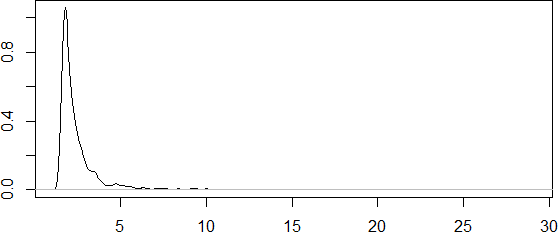
\includegraphics[width=0.8\textwidth]{rytgaard1990/predictive_Y_f.png}
\caption{Estimated Predictive PDF of \( Y_f \)}
\label{fig:9}
\end{figure}

The inverse CDF method was also used to estimate the predictive distribution of \( S_f \), representing a future observation of \( S_t \). The procedure was as follows: 1{,}000 values were drawn from the posterior predictive distribution of \( N_f \). For each uniformly drawn \( U \), a Poisson sample was generated using each posterior value of \( \theta^{(i)} \), and the average of these samples was computed and rounded to obtain \( N_f \). Then, for each simulated value of \( N_f \), that many samples were drawn from the predictive distribution of \( Y_f \) (as described earlier), and the resulting values were summed to obtain a draw of \( S_f \).

Figure~\ref{fig:10} presents the histogram of the resulting \( S_f \) samples, along with the estimated density and three fitted distributions using moment matching. As observed by Dudley, the Gamma distribution provides the best fit. The fitted Gamma distribution has parameters \( \alpha = 2.435 \) and \( \beta = 0.292 \).

\begin{figure}[!ht]
\centering
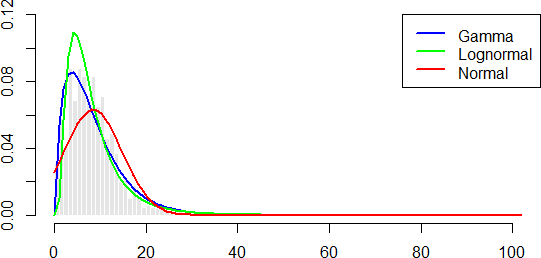
\includegraphics[width=0.8\textwidth]{rytgaard1990/predictive_S_f.png}
\caption{Histogram and Fitted Distributions for Predictive \( S_f \)}
\label{fig:10}
\end{figure}

Table~\ref{tab:7} shows various percentiles of the simulated \( S_f \) values. The distribution exhibits a suitably long tail, which aligns with expectations for a heavy-tailed claim size distribution. This indicates that the simulation method used was effective in generating large \( Y \) values, thereby capturing the tail behavior of the predictive distribution of \( S \) more accurately. Proper representation of the tail is important, as most aggregate claims are moderate, but extreme values can occasionally occur.

\begin{table}[!ht]
\centering
\footnotesize
\setlength{\tabcolsep}{5pt}
\caption{Percentiles of Simulated \( S_f \) Values}
\label{tab:7}
\begin{tabular}{
>{\raggedright\arraybackslash}p{\widthof{99th Percentile}}
S[table-format=2.3]
}
\hline
\textbf{Percentile} & \textbf{Value} \\ 
\hline
Median & 7.630 \\ 
90th Percentile & 15.170 \\
95th Percentile & 18.103 \\
99th Percentile & 26.410 \\
Maximum & 35.851 \\
\hline
\end{tabular}
\end{table}

\printbibliography{references}
\end{document}